%
%  Halitosis
%
%  Created by Martell on 2012-05-08.
%  Copyright (c) 2012 UBC Fisheries Centre. All rights reserved.
%
\documentclass[12pt]{article}

% Use utf-8 encoding for foreign characters
\usepackage[utf8]{inputenc}

% Setup for fullpage use
\usepackage{fullpage}

% Uncomment some of the following if you use the features
%
% Running Headers and footers
%\usepackage{fancyhdr}

% Multipart figures
%\usepackage{subfigure}

% More symbols
\usepackage{amsmath}
\usepackage{amssymb}
\usepackage{latexsym}

% Surround parts of graphics with box
\usepackage{boxedminipage}

% Package for including code in the document
\usepackage{listings}

% If you want to generate a toc for each chapter (use with book)
\usepackage{minitoc}

% This is now the recommended way for checking for PDFLaTeX:
\usepackage{ifpdf}

%\newif\ifpdf
%\ifx\pdfoutput\undefined
%\pdffalse % we are not running PDFLaTeX
%\else
%\pdfoutput=1 % we are running PDFLaTeX
%\pdftrue
%\fi

\ifpdf
\usepackage[pdftex]{graphicx}
\else
\usepackage{graphicx}
\fi
\title{An equilibrium model for exploring discard and wastage in Pacific Halibut}
\author{ Steven Martell }

\date{2012-05-08}

\begin{document}

\ifpdf
\DeclareGraphicsExtensions{.pdf, .jpg, .tif}
\else
\DeclareGraphicsExtensions{.eps, .jpg}
\fi

\maketitle


\begin{abstract}
	The practice of discarding prohibited species and discarding of undersized fish has implications for the future spawning biomass and yield in the directed fishery.  An equilibrium model is used to explore the cumulative effects of size-selective fishing on the lost yield in directed fisheries and lost mature spawning biomass.
\end{abstract}

\section{Introduction} % (fold)
\label{sec:introduction}
In this paper, I derive an equilibrium model for exploring the implications of size-selective fisheries that use minimum size limits.  The model accounts for variability in length-at-age,  the cumulative effects of size-selective fishing, and a joint probability model to account for retention and discard mortality.
% section introduction (end)

\section{Methods} % (fold)
\label{sec:methods}
In an age-structure model the equilibrium yield is the sum over all ages of the biomass-at-age multiplied by the fraction of age-specific mortality associated with fishing:
\begin{equation}\label{eq:1}
	Y_e = \sum_{a=1}^\infty  \frac{ B_{a,e} F_{a,e}[1-\exp(-M_a-F_{a,e})] }{ M_a + F_{a,e} },
\end{equation}
where $F_{a,e} = f_e v_a$, or the fully selected fishing mortality rate $f_e$ times the age-specific selectivity $v_a$.  Biomass-at-age is the product of the numbers-at-age ($N_a$) times the average weight-at-age ($w_a$). Assuming a steady-state (equilibrium) unfished condition the biomass-at-age can be expressed as the survivorship-at-age, mean weight-at-age and the number of unfished age-1 recruits ($R_o$).  For unfished conditions the survivorship is calculated using the following recursive equation:
\begin{equation}\label{eq:2}
l_a = \begin{cases}
    1, &\quad a=1\\
    l_{a-1}\exp(-M_{a-1}), &\quad a>1.\\
\end{cases}
\end{equation}
Note that if there are notable sex-specific differences in natural mortality rates and growth rates, another dimension in the survivorship and weigth-at-age arrays is required. For example, the yield equation in \eqref{eq:1} would include an additional summation over gender and sex-specific biomass-at-age, fishing and natural mortality rates. Indices for gender are omitted in the notation for the sake of clarity.

The age-specific biomass is then given by:
\begin{equation}\label{eq:3}
	B_{a,e} = R_o l_a w_a.
\end{equation}

For mathematical convenience a series of per-recruit incidence functions are used to compute total biomass per recruit, spawning biomass per recruit, yield per recruit, etc. using $\phi_{x}$ where the subscript $x$ denotes they type of incidence function.  Note that hereafter, I use uppercase subscripts to denote unfished conditions and lowercase subscripts to denote fished conditions.   For example the unfished spawning biomass per recruit is defined as:
\begin{equation}\label{eq:4}
	\phi_{B} = \sum_{a=1}^\infty l_a m_a w_a,
\end{equation}
where $m_a$ is the proportion mature-at-age. The use of these incidence functions greatly simplifies the math in the subsequent calculations in that it is now possible to calculate total population abundance, spawning abundance, total yield etc. using an estimate of equilibrium recruitment.  For example, the unfished spawning biomass is denoted as $B_o = R_o \phi_B$.

Expressing the catch equation as a sum over ages of biomass that is vulnerable to harvest is given by:
\begin{equation}\label{eq:5}
	Y_e = f_e R_e \sum_{a=1}^\infty \frac{l_a v_a w_a [1-\exp(-M_a-f_e v_a)]}
	{M_a+f_e v_a}.
\end{equation}
Note that the summation term in \eqref{eq:5} can be represented as an incidence function, namely:
\begin{equation}\label{eq:6}
	\phi_y = \sum_{a=1}^\infty \frac{l_a v_a w_a [1-\exp(-M_a-f_e v_a)]}
	{M_a+f_e v_a},
\end{equation}
and the yield equation reduces to:
\begin{equation}\label{eq:7}
	Y_e = f_e R_e \phi_y
\end{equation}

For a given steady-state fishing mortality rate $f_e$, the long-term equilibrium recruitment that would result from the reduced spawning biomass $B_e$ is a function of the steepness of the stock recruitment relationship (i.e., compensation in juvenile survival rates).  For the Beverton-Holt stock-recruitment model, recruitment is defined as:
\begin{equation}\label{eq:8}
	R_e = \frac{a B_e}{1+b B_e},
\end{equation}
where $a$ is the maximum number of recruits per unit of spawning biomass (or the slope at the orign) which can be defined as a multiple $k$ of the unfished recruits per spawner, or $a = kR_o/Bo$.  Substituting $B_o = R_o \phi_B$ into the previous expression the $a$ parameter simplifies to $a=k/\phi_B$. Solving \eqref{eq:8} for $b$, substituting $R_o \phi_B$ for $B_o$, simplifies to $b=(k-1)/(R_o\phi_B)$.  Given these relationships, the Beverton-Holt model can be re-written as:
\begin{equation}\label{eq:9}
	R_e = \dfrac{\frac{k}{\phi_B}B_e}{1+\frac{(k-1)}{R_o\phi_B}B_e}
	    = \dfrac{\frac{k}{\phi_B}R_e\phi_b}{1+\frac{(k-1)}{R_o\phi_B}R_e\phi_b}.
\end{equation}
Note here that the subscripts ($_o$, $_B$) and ($_e$, $_b$) denote unfished and fished conditions.  Equation \ref{eq:9} further simplifies to:
\begin{equation}\label{eq:10}
	R_e = \frac{R_o(k-\phi_B/\phi_b)}{k-1},
\end{equation}
where $\phi_b$ is the spawning biomass under fished conditions.  To calculate the spawning biomass under fished conditions, the age-specific survivorship curve is modified to include the effects of steady-state fishing mortality:
\begin{equation}\label{eq:11}
	l_a^{(f)} = \begin{cases}
	    1, &\quad a=1\\
	    l_{a-1}^{(f)}\exp(-M_{a-1}-f_e v_{a-1}), &\quad a>1.\\
	\end{cases}
\end{equation}
Thus, the unfished and fished biomass per recruit is given as:
 \[
 \phi_B = \sum_{a=1}^\infty l_a m_a w_a, \quad
 \phi_b = \sum_{a=1}^\infty l_a^{(f)} m_a w_a.
 \]
In summary, \eqref{eq:10} and \eqref{eq:11} permit the calculation of equilibrium recruitment under fished conditions and only require initial estimates of global scale (e.g., unfished recruitment), rate parameters ($M$ and the recruitment compensation ratio $k$, or steepness), and age-schedule information on weight-at-age and maturity-at-age.  For a given steady-state fishing mortality rate $f_e$, the equilibrium yield can be calculated using \eqref{eq:7}, and similarly, the equilibrium spawning biomass can be calculated using:
\begin{equation}\label{eq:12}
	B_e = R_e \phi_b
\end{equation}

\subsection{Accounting for discard mortality} % (fold)
\label{sub:accounting_for_discard_mortality}
In cases where fish must be legally discarded due to size limits or prohibited species catch, accounting for the affects of non-zero discard mortality rates requires a joint probability model where: (1) there is a probability of capturing a fish of a given age/length, and (2) a probability of retaining an age-$a$ fish given its length.  To account for discard mortality in the above catch equations, the age-specific vulnerability term $v_a$ can be modified to account for retention and discard components.  Specifically, vulnerability-at-age can be represented as:
\begin{equation}\label{eq:13}
	v_a = s_a [r_a+(1-r_a)d_a]
\end{equation}
where $s_a$ is a age-specific probability of capturing a fish of a given age $a$ (selectivity), $r_a$ is the probability of retaining a fish of a given age $a$ which is equal to the probability of a fish being larger than the minimum size limit ($r_a=p(l_a)>\mathrm{MSL}$), and $d_a$ is the average age-specific discard mortality rate.  Note that if $d_a=0$, the assumption is that all released fish survive and are available for recapture in the future.  To determine what proportion of age-$a$ fish are greater than the minimum size limit, it is assumed that length-at-age has a normal distribution and the cumulative normal probability density is used to approximate $p(l_a)>\mathrm{MSL}$:
\begin{equation}\label{eq:14}
	r_a = \int_{l=\mathrm{MSL}}^{l=\infty} \frac{1}{\sigma_a\sqrt{2\pi}} 
	\exp\left(-\frac{(l-l_a)^2}{2\sigma_a^2} \right)dl
\end{equation}
Equation \ref{eq:14} is the area under a normal curve with a mean corresponding to the mean length-at-age ($l_a$) and the standard deviation in length-at-age ($\sigma_a$) starting at the minimum size limit up to an infinite size.
% subsection accounting_for_discard_mortality (end)

\subsection{Cumulative effects of size selective fishing} % (fold)
\label{sub:cumulative_effects_of_size_selective_fishing}
To represent the variation in growth rates and the cumulative effects of size selective fishing, we assume that the population consists of a number of distinct groups ($G$) that vary in the asymptotic length.  The underlying assumption is that in a given population, the asymptotic length ($l_\infty$) has a normal distribution with a coefficient of variation equal to 0.1.  A total of 11 distinct groups are are modelled with the corresponding lower and upper mean $l_\infty$ set at $\pm$ 1.97 times the standard deviation in $l_\infty$.  We further assume that the proportion of total future recruitment to each of these $G$ groups is normally distributed ($p_g$) irrespective of the composition of the spawning population (i.e., we assume no genetic effects associated with size-selective fishing).  The incidence functions ($\phi$) in the above equations are then modified to sum over both ages and the growth groups to represent the per recruit processes, for example, spawning biomass per recruit is given by:
\begin{equation}\label{eq:15}
	\phi_B = \sum_g p_g \sum_{a=1}^{a=\infty} l_a w_a m_a.
\end{equation}
Using the structural assumption defined in \eqref{eq:15}, faster growth fish would theoretically recruit to the size limit earlier in life (or a higher proportion of that age-class would be vulnerable to retention and selectivity) and have an overall highter total mortality rate in comparison to slower growing individuals.  The accounting of equilibrium yield and spawning biomass then proceeds using \eqref{eq:7} and \eqref{eq:12} with the differential mortality rates for faster and slower growing individuals.

% subsection cumulative_effects_of_size_selective_fishing (end)

\subsection{Calculation of yield loss and spawning biomass loss ratios} % (fold)
\label{sub:calculation_of_yield_loss_and_spawning_biomass_loss_ratios}

The yield loss ratio is defined as the difference between the yield obtained with no discard mortality (all discarded fish survive) and the yield obtained with discard mortality rate $d_a>0$ per pound of dead fish discarded.  For any combination of fishing mortality $f_e$ and minimum size limit, the yield loss ratio is calculated as:
\begin{equation}\label{eq:16}
	\mathrm{YLR} = \frac{Y_e^{d_a=0} - Y_e^{d_a=0.16}}{D_e^{d_a=0.16}},
\end{equation}
where $D_e^{d_a=0.16}$ is the total amount discarded fish that are assumed to die under a discard mortality rate of 0.16 yr$^{-1}$. In the case of \eqref{eq:16}, the equilibrium yield refers specifically to the retained portion of the catch and not the component associated with discarding. The retained yield and dead discards are computed as follows:
\begin{align}
	Y_e^{d_a=0.16} &= f_e R_e \phi_y, \quad \mbox{where} \label{eq:17}\\
	 \phi_y &=  \sum_{a=1}^\infty 
	\frac{l_a s_a r_a w_a [1-\exp(-M_a-f_e s_a [r_a+(1-r_a)d_a])]}
	{M_a+f_e s_a [r_a+(1-r_a)d_a]} \nonumber \\[2ex]
	D_e^{d_a=0.16} & = f_e R_e \phi_d, \quad \mbox{where}\label{eq:18}\\
	\phi_d &=  \sum_{a=1}^\infty 
	\frac{l_a s_a (1-r_a)d_a w_a [1-\exp(-M_a-f_e s_a [r_a+(1-r_a)d_a])]}
	{M_a+f_e s_a [r_a+(1-r_a)d_a]} \nonumber 
\end{align}
In \eqref{eq:17} and \eqref{eq:18} the $\phi_y$ and $\phi_d$ terms correspond to the retained yield per recruit and the dead discards per recruit, respectively.  Note that in \eqref{eq:17} when the discard mortality rate $d_a=0$, the mortality associated with fishing is only on the retained component as all discarded animals are assumed to survive.

The spawning biomass ratio is defined as the difference between the spawning biomass obtained with no discard mortality (all discarded fish survive) and the spawning biomass obtained with a discard mortality rate $d_a>0$ per pound of dead fish discarded. Again, for any combination of fishing mortality $f_e$ and minimum size limit, the spawning biomass loss ratio is calculated as:
\begin{equation}\label{eq:19}
	\mathrm{BLR} = \frac{B_e^{d_a=0}-B_e^{d_a=0.16}}{D_e^{d_a=0.16}},
\end{equation}
where $B_e^{d_a=0.16}$ is the mature female biomass (subscript for sex ignored for clarity) with a fishery discard mortality rate of 0.16 yr$^{-1}$.  The equilibrium spawning biomass is given by:
\begin{align}
	B_e^{d_a=0.16}&=R_e \phi_b \quad \mbox{where,}\label{eq:20}\\
	\phi_b & = \sum_{a=1}^\infty l_a^{(f)} m_a w_a \nonumber, 
\end{align}
where $l_a^{(f)}$ includes the effects of discard mortality in the recursive survivorship calculation.  
% subsection calculation_of_yield_loss_and_spawning_biomass_loss_ratios (end)
% section methods (end)

\section{Results} % (fold)
\label{sec:results}
Under the current 2011 growth (or what ever should be in the table of growth parameters) the expected yield loss ratio for each pound of dead discarded fish is slightly less than 1 pound under the current 32 inch size limit and a target fully selected fishing mortality rate of 0.215 (Figure \ref{fig:fig:Halitosis:SlowGrowth}a).  The expected loss in female spawning biomass per pound of discarded fish is slightly less than 4.5 pounds under the same 32 inch size limit and fishing mortality rate of 0.215 (Figure \ref{fig:fig:Halitosis:SlowGrowth}b).

If growth rates continue to decline where asymptotic lengths are 80\% of the current values, the expected yield loss ratio is reduced by nearly 60\% to 0.4 pounds per pound of dead discarded fish less than the minimum size limit (Figure \ref{fig:fig:Halitosis:SlowGrowth}c).  Similarly, the expected female spawning biomass loss per pound of dead discarded undersized fish declines to less than 4 pounds (Figure \ref{fig:fig:Halitosis:SlowGrowth}d).

\begin{figure}[htbp]
	\centering
		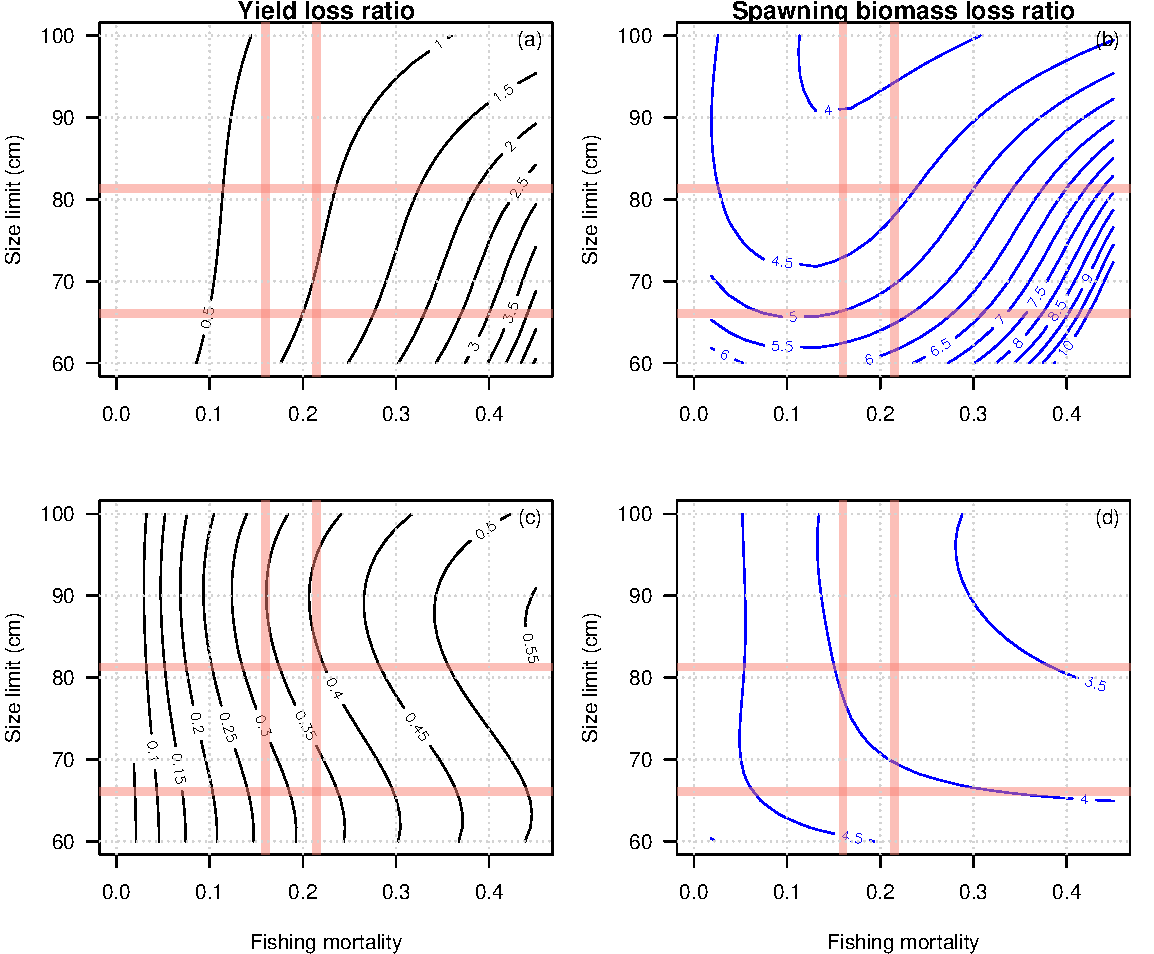
\includegraphics[width=0.9\textwidth]{fig:Halitosis:SlowGrowth.pdf}
	\caption{Isopleths of yield loss and female spawning biomass ratios per pound of discarded dead Pacific halibut under alternative steady-state fishing mortality rates and minimum size limits in the directed fishery.  Vertical shaded bars correspond to fishing mortality rates of 0.16 and 0.215, and horizontal shaded bars correspond to 26 and 32 inch minimum size limits.}
	\label{fig:fig:Halitosis:SlowGrowth}
\end{figure}

% section results (end)

\bibliographystyle{plain}
\bibliography{}
\end{document}
